\documentclass[dvipdfmx]{jsarticle}
\usepackage{graphics}
\usepackage{amsmath}
\usepackage{amssymb}
\usepackage{amsthm}
\usepackage{mathtools}
\usepackage{ascmac}
\usepackage{bm}
\usepackage{url}
\usepackage{txfonts}
\usepackage{docmute}
\usepackage{color}
\usepackage{tikz}
\usepackage{docmute}
\usetikzlibrary{calc}
\usetikzlibrary{intersections}

\usepackage{qexam}

\title{証明問題の書き方}
\author{}
\date{}

\begin{document}
	\maketitle
	本資料では平面図形の証明問題の例題とその解答例を紹介する.
	扱う問題はすべて「中学校数学・学習サイト」に掲載されている
	問題,または改題したものである.
	答案に関してはサイトに示したものと異なる.

	\url{https://math.005net.com}

	\documentclass[dvipdfmx]{jsarticle}
\usepackage{graphics}
\usepackage{amsmath}
\usepackage{amssymb}
\usepackage{amsthm}
\usepackage{mathtools}
\usepackage{ascmac}
\usepackage{bm}
\usepackage{url}
\usepackage{txfonts}
\usepackage{color}

\usepackage{tikz}
\usetikzlibrary{calc}
\usetikzlibrary{intersections}

\begin{document}
	\section{図形の性質}
	証明問題を扱う前に図形の性質について述べる.図形の性質の理解が
	証明問題を解く上での重要な鍵になる.
	\subsection{等しい角度}
	角度が等しいことがわかるケースを挙げると次の通りとなる.
	\begin{itemize}
		\item 対頂角
		\item 平行線の同位角・錯角
		\item 共通の角
		\item 平行四辺形の向かい合った角
		\item 二等辺三角形の底角
		\item 等脚台形の上底,または下底の両端角
		\item 円周角の定理
		\item 計算
	\end{itemize}
	4つ目以降は馴染みのない条件となっているはずだ.この他にも角が等しいケースはあるが,
	これくらいは頭に置いておきたい.これらを2つずつ紹介する.

	\subsubsection{対頂角}
	対頂角は2直線が交差するときに生まれる角度の関係である.
	図\ref{tikz_taityokaku}のように2直線の間の角が等しくなる.
	最も基本的な性質である.


	\begin{figure}[htbp]
		\centering
		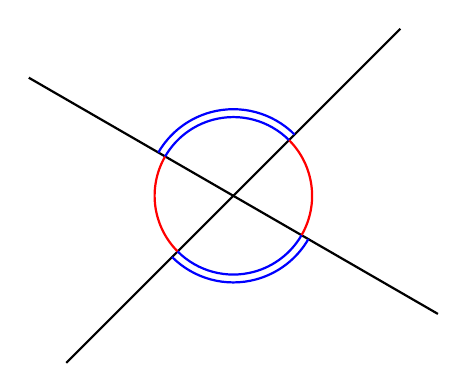
\begin{tikzpicture}[scale=1]
			\draw[thick]($(0, 0)-(45:3)$)--($(0, 0)+(45:3)$);
			\draw[thick]($(0, 0)-(-30:3)$)--($(0, 0)+(-30:3)$);

			\draw[thick, red]($(0, 0)+(-30:1)$) arc[radius=1, start angle=-30, end angle=45];
			\draw[thick, red]($(0, 0)-(-30:1)$) arc[radius=1, start angle=150, end angle=225];

			\draw[thick, blue]($(0, 0)+(45:1)$) arc[radius=1, start angle =45, end angle=150];
			\draw[thick, blue]($(0, 0)+(45:1.1)$) arc[radius=1.1, start angle =45, end angle=150];

			\draw[thick, blue]($(0, 0)-(45:1)$) arc[radius=1, start angle =225, end angle=330];
			\draw[thick, blue]($(0, 0)-(45:1.1)$) arc[radius=1.1, start angle =225, end angle=330];
		\end{tikzpicture}
		\caption{対頂角}
		\label{tikz_taityokaku}
	\end{figure}

	\subsubsection{平行線の同位角と錯角}
	平行線の錯角は2本の平行な直線の両方に交わる直線があるときに
	生じる角度の関係である.図\ref{tikz_heikosen_doikaku_sakkaku}の
	ように2つの箇所で同じような
	位置関係にある角度が等しくなるのが同位角の関係(赤一重)である.
	錯角(青二重)も何ら難しいものではない.
	
	\begin{figure}[htbp]
		\centering
		\begin{tikzpicture}[scale=1]
			% \draw[very thin, gray, dashed](-5, -5)grid(5, 5);

			\draw[thick, name path=lower_line] (-5, -2)--(5, -2);
			\draw[thick, name path=upper_line] (-5, 2)--(5, 2);

			\draw[thick, name path=line](60:-4)--(60:4);

			\draw[red, name intersections={of=lower_line and line, by={lower_point}}]($(lower_point)+(0:0.5)$)arc[radius=0.5, start angle=0, delta angle=60];
			\draw[red, name intersections={of=upper_line and line, by={upper_point}}]($(upper_point)+(0:0.5)$)arc[radius=0.5, start angle=0, delta angle=60];

			\draw[thick, blue]($(lower_point)+(60:0.5)$)arc[radius=0.5, start angle=60, delta angle=120];
			\draw[thick, blue]($(upper_point)+(0:0.5)$)arc[radius=0.5, start angle=0, delta angle=-120];
			\draw[thick, blue]($(lower_point)+(60:0.6)$)arc[radius=0.6, start angle=60, delta angle=120];
			\draw[thick, blue]($(upper_point)+(0:0.6)$)arc[radius=0.6, start angle=0, delta angle=-120];
		\end{tikzpicture}
		\caption{平行線の同位角と錯角}
		\label{tikz_heikosen_doikaku_sakkaku}
	\end{figure}

	\subsubsection{共通の角}
	最も簡単なのは共通の角である.しかし,以外にも忘れることが
	あるので注意が必要である.また,証明のときは書いたほうが
	いいのかという疑問を持つかもしれないが,必ず書くことを勧める.
	何かが等しいということを言うときは簡単であっても理由を書く
	こと
	\footnote{明らかなことであるときは,
	明らかであると言うことも大事.}を癖付けよう.

	\subsubsection{平行四辺形の向かい合った角}
	平行四辺形では向かい合った角が等しい.これは実際に
	問題で使うことがあるのか怪しい条件だが,1度だけお目にかかったので
	紹介する.

	他にも平行四辺形の隣り合った角の和が180度であったり,
	平行四辺形の条件を利用する問題はないわけではない.
	2組の平行な直線があれば,それらで平行四辺形ができるので
	そのような場合は注意しよう.

	\subsubsection{二等辺三角形の底角}
	これはみんなもよく知るところの条件だろう.
	図\ref{tikz_nitohen_tekaku}のように二等辺三角形の底角は等しい.

	\begin{figure}[htbp]
		\centering
		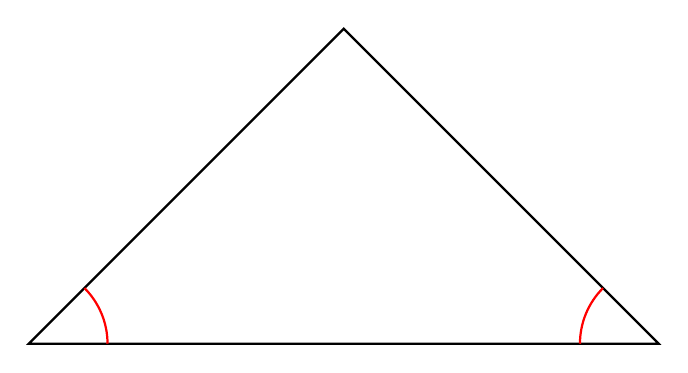
\begin{tikzpicture}[scale=2]
			\draw[thick](0, 0)--(4, 0)--(2, 2)--cycle;
			\draw[thick, red](0.5, 0)arc[radius=0.5, start angle=0, end angle=45];
			\draw[thick, red](3.5, 0)arc[radius=0.5, start angle=180, delta angle=-45];
		\end{tikzpicture}
		\caption{二等辺三角形の底角}
		\label{tikz_nitohen_tekaku}
	\end{figure}

	\subsubsection{等脚台形}
	等脚台形は二等辺三角形を底辺と平行な直線で
	切った図形である.図\ref{tikz_tokyakudaikei}が等脚台形である.
	もとが二等辺三角形であるから下底の両端の角が等しいのは明らかだ.
	上底に関しても等しいことは切り取った三角形が二等辺三角形
	であることからすぐにわかる.

	\begin{figure}[htbp]
		\centering
		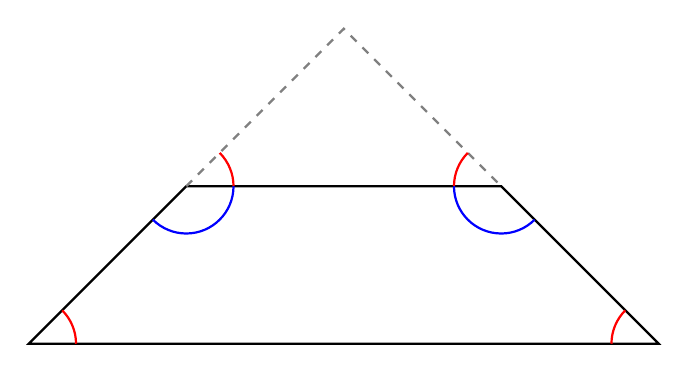
\begin{tikzpicture}[scale=2]
			\draw[thick](0, 0)--(4, 0)--(3, 1)--(1, 1)--cycle;
			\draw[thick, gray, dashed](1, 1)--(2, 2)--(3, 1);
			\draw[thick, red](0.3, 0)arc[radius=0.3, start angle=0, end angle=45];
			\draw[thick, red](3.7, 0)arc[radius=0.3, start angle=180, delta angle=-45];

			\draw[thick, red](1.3, 1)arc[radius=0.3, start angle=0, end angle=45];
			\draw[thick, red](2.7, 1)arc[radius=0.3, start angle=180, delta angle=-45];

			\draw[thick, blue](1.3, 1)arc[radius=0.3, start angle=0, delta angle=-135];
			\draw[thick, blue](2.7, 1)arc[radius=0.3, start angle=180, delta angle=135];
		\end{tikzpicture}
		\caption{等脚台形}
		\label{tikz_tokyakudaikei}
	\end{figure}

	\subsubsection{円周角の定理}
	円周角の定理はある円に対しては同じ長さ
	\footnote{同じ弧である必要はない.
	大事なのはこの長さと円周角が対応しているという理解である.}
	の弧に対する
	円周角が等しいことを示している.

	円周角の定理の利用のときは,必ずどの点を通る円なのかを
	明らかにしなければならない.
	具体的には例題を扱うときに述べる.

	円周角の定理を使う円はたいてい自らの力で見つける必要が
	あるので,これが思いつかないことで問題が解けなくなる
	という状況を散見する.

	\subsection{計算}
	なんとも漠然とした話であるが計算によって同じ角である
	というのが入試問題では必ず出てくる.
	最もよく見るケースをここで紹介する.

	図\ref{tikz_onajikaku_hiku}は2組の直角な角が頂点を共有して
	ずれるように配置されている.
	すると赤の角度は両方とも90度から青の角を引いたものとなっている.
	つまり,同じ角度なのだ.


	\begin{figure}[htbp]
		\centering
		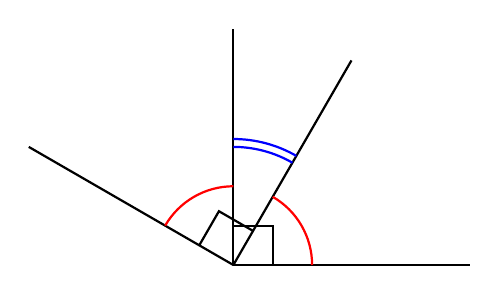
\begin{tikzpicture}[scale=1]
			\draw[thick](0, 0)--(0:3);
			\draw[thick](0, 0)--(90:3);
			\draw[thick](0, 0)--(60:3);
			\draw[thick](0, 0)--(150:3);
			\draw[thick](0:0.5)--($(0:0.5)+(90:0.5)$)--(90:0.5);
			\draw[thick](60:0.5)--($(60:0.5)+(150:0.5)$)--(150:0.5);

			\draw[thick, red](0:1)arc[radius=1, start angle=0, end angle=60];
			\draw[thick, red](90:1)arc[radius=1, start angle=90, end angle=150];
			\draw[thick, blue](60:1.5)arc[radius=1.5, start angle=60, end angle=90];
			\draw[thick, blue](60:1.6)arc[radius=1.6, start angle=60, end angle=90];
		\end{tikzpicture}
		\caption{同じ角を引く}
		\label{tikz_onajikaku_hiku}
	\end{figure}


	このようなケースは角度が数値としてわかるものが
	複数ある場合に現れる.同じ数値から同じ角度を引けば,
	当然残る角も等しくなるという流れだ.


	\subsection{等しい長さ}
	辺が等しくなる場合は円の半径である場合と,共通な辺の場合だけである.
	そのため,いちいち説明することはない.

	\subsection{辺の比}
	辺の長さの比が同じ場合はあまりない.辺の長さが数値としてわかっていない場合は
	必ず平行線が関係してくる.まず,一番簡単に現れるケースは図\ref{tikz_heikosen_senbun_hi}のような状態である.
	3本の平行線とそれらに交わる直線があると必ず線分の長さの比は等しくなる.

	逆に辺の長さの比が等しいことから,3本の横線が平行であると言うこともできる
	\footnote{並行の証明自体があまり出てこないので使うことは少なめ.}.



	\begin{figure}[htbp]
		\centering
		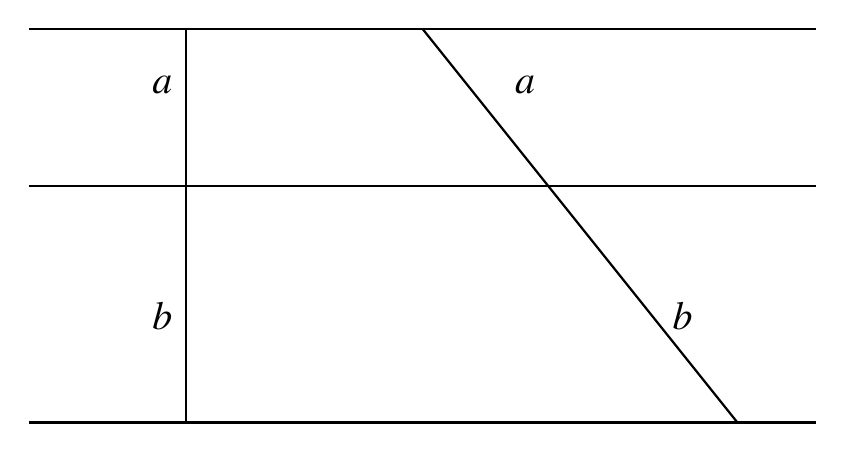
\begin{tikzpicture}[scale=1]\Large
			
			\draw[thick] (-5, 2)--(5, 2);
			\draw[thick] (-5, 0)--(5, 0);
			\draw[thick] (-5, -3)--(5, -3);

			\draw[thick] (-3, 2)--(-3, -3);
			\draw[thick] (0, 2)--(4, -3);

			\node[above left] at (-3, 1){$a$};
			\node[above left] at (-3, -2){$b$};

			\node[above right] at (1, 1){$a$};
			\node[above right] at (3, -2){$b$};
		\end{tikzpicture}
		\caption{平行線による線分の比}
		\label{tikz_heikosen_senbun_hi}
	\end{figure}

	平行線が関わるケースで重要なのは三角形の底辺とその平行な線である.
	図\ref{tikz_sannkakukei_teihenn_heiko}は三角形の底辺に対して平行な線が引いてある.
	すると同じ辺の長さの比が3ヶ所に現れる.
	要注意なケースである.

	こちらでも,辺の比が等しいことから線分が平行であると言うことができる.

	\begin{figure}[htbp]\Large
		\centering
		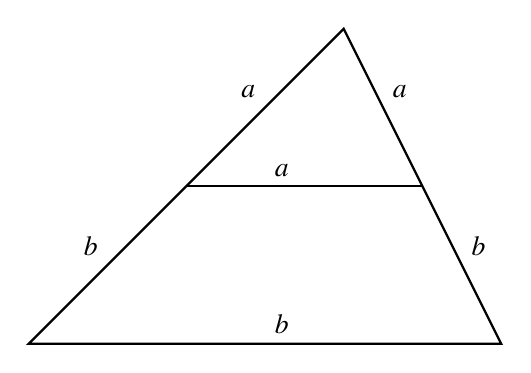
\begin{tikzpicture}[scale=1]
			\draw[thick] (-3, 0)--(3, 0)--(1, 4)--cycle;
			\draw[thick] (-1, 2)--(2, 2);

			\node[above left] at (0, 3){$a$};
			\node[above left] at (-2, 1){$b$};

			\node[above right] at (1.5, 3){$a$};
			\node[above right] at (2.5, 1){$b$};

			\node[above right] at (0, 2){$a$};
			\node[above right] at (0, 0){$b$};
		\end{tikzpicture}
		\caption{三角形の底辺と平行な線分}
		\label{tikz_sannkakukei_teihenn_heiko}
	\end{figure}


	さらに,辺の比がわかる最も重要なケースは角の二等分線が関係するときである.
	図\ref{tikz_kaku_nitobunsenn_hi}のように,三角形の1つの頂点から引かれる角の二等分線が向かい合う辺に
	交わると,それによって分かれる2つの部分の比がわかるのだ.

	\begin{figure}[htbp]
		\centering
		\begin{tikzpicture}[scale=2]\Large

			\draw[white, name path=circ1](3, 0) arc(0:33:6);
			\draw[white, name path=circ2](0, 0) arc(180:100:3);
			\draw[thick, name intersections={of=circ1 and circ2, by={a}}](a)--(-3, 0)--(3, 0)--cycle ;
			\draw[thick] (a)--(1, 0);

			\node[above left] at ($(a)!0.5!(-3, 0)$) {$a$};
			\node[above right] at ($(a)!0.5!(3, 0)$) {$b$};

			\node[below left] at ($(1, 0)!0.5!(-3, 0)$) {$a$};
			\node[below right] at ($(1, 0)!0.5!(3, 0)$) {$b$};
		\end{tikzpicture}
		\caption{角の二等分線と線分の比}
		\label{tikz_kaku_nitobunsenn_hi}
	\end{figure}

	角の二等分線と出てきたら必ず疑うべき条件である.見落としは許されない.

	\subsection{証明に用いる定理}
	図形問題の一部では定理を用いるものがある.
	中学数学で扱う定理を紹介する.

	\subsubsection{円周角の定理}
	説明はすでにしている.図\ref{tikz_enshukaku_teiri}で表される等しい角の関係である.
	また,円周角は中心角の半分であるという性質を忘れては
	ならない.

	\begin{figure}[htbp]
		\centering
		\begin{tabular}{c}
			\begin{minipage}{0.45\hsize}
				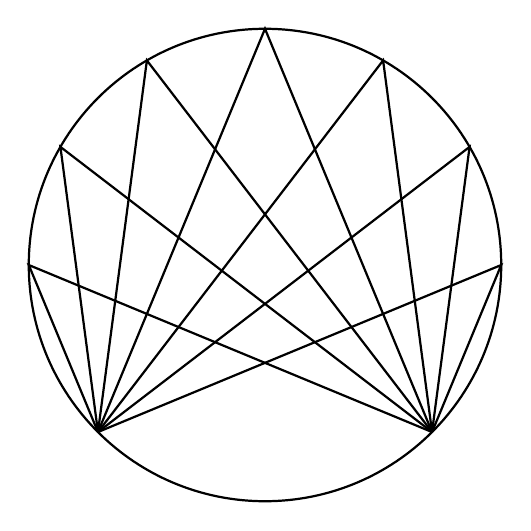
\begin{tikzpicture}[scale=1]
					\draw[thick] (0, 0)circle[radius=3];
					\coordinate(a) at (225:3) ;
					\coordinate(b) at (-45:3) ;
					\foreach \x in {0, 30, ..., 180}{
						\draw[thick] (a)--(\x:3)--(b);
					}
				\end{tikzpicture}
			\end{minipage}

			\begin{minipage}{0.45\hsize}
				
\begin{tikzpicture}[scale=1]
					\draw[thick] (0, 0)circle[radius=3];
					\coordinate(a) at (225:3) ;
					\coordinate(b) at (-45:3) ;
					\draw[thick] (a)--(100:3)--(b);
					\draw[thick] (a)--(0, 0)--(b);
					\fill (0, 0)circle (2pt);
				\end{tikzpicture}
			\end{minipage}
		\end{tabular}
		\caption{円周角の定理}
		\label{tikz_enshukaku_teiri}
	\end{figure}

	\subsubsection{中点連結定理}
	三角形の2辺の中点を結ぶ線分は,他の辺と並行であり
	長さは半分であるという定理である.
	今は
	\begin{gather*}
		\mathrm{AM}=\mathrm{BM}\\
		\mathrm{AN}=\mathrm{BN}\\
	\end{gather*}
	となっている.すると,
	\begin{gather*}
		\mathrm{MN}= \frac{1}{2}\mathrm{BC}, \quad 
		\mathrm{MN}//\mathrm{BC}
	\end{gather*}
	であることが中点連結定理から直ちにわかる.

	\begin{figure}[htbp]\Large
		\centering
		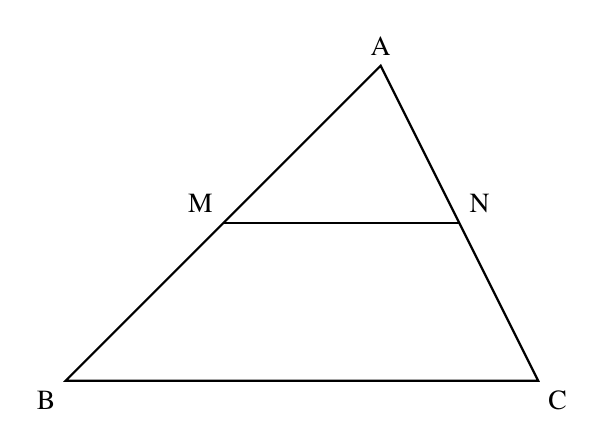
\begin{tikzpicture}[scale=1]
			\draw[thick] (-3, 0)node[below left]{B}--(3, 0)node[below right]{C}--(1, 4)node[above]{A}--cycle;
			\draw[thick] (-1, 2)node[above left]{M}--(2, 2)node[above right]{N};
		\end{tikzpicture}
		\caption{三角形の底辺と平行な線分}
		\label{tikz_tyutenrenketu_teiri}
	\end{figure}

	\subsection{三平方の定理}
	直角三角形に成立する辺の長さに関する定理である.
	図\ref{tikz_sannheihou_teiri}の直角三角形に対して次の式が成立する.
	\[\mathrm{AC}^2=\mathrm{AB}^2+\mathrm{BC}^2\]

	\begin{figure}[htbp]
		\centering
		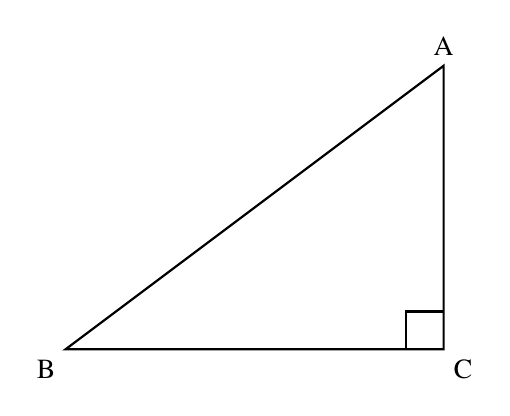
\begin{tikzpicture}[scale=1.2]
			\draw[thick] (0, 0)node[below left]{B}--(4, 0)node[below right]{C}--(4, 3)node[above]{A}--cycle;
			\draw[thick] (3.6, 0)--(3.6, 0.4)--(4, 0.4);
		\end{tikzpicture}
		\caption{三平方の定理}
		\label{tikz_sannheihou_teiri}
	\end{figure}

	定理の証明はネットに溢れているので自ら調べてみよう.

\end{document}

	\documentclass[dvipdfmx]{jsarticle}
\usepackage{graphics}
\usepackage{amsmath}
\usepackage{amssymb}
\usepackage{amsthm}
\usepackage{ascmac}
\usepackage{bm}
\usepackage{url}
\usepackage{txfonts}
\usepackage{color}
\usepackage{tikz}
\usetikzlibrary{calc}
\usetikzlibrary{intersections}

\usepackage{qexam}

\begin{document}

	\section{三角形の合同}
	三角形の合同の証明を扱う節である.ここで型を覚えると,
	記述に困ることはなくなる.
	\subsection{合同の条件}
	はじめに,合同の条件をまとめておく.
	\begin{itemize}
		\item 三角形の3辺の長さがそれぞれ等しい.
		\item 三角形の2辺の長さと,そのあいだの角がそれぞれ等しい.
		\item 三角形の1辺の長さと,その両端の角がそれぞれ等しい.
		\item 直角三角形の斜辺の長さと,他の1辺の長さがそれぞれ等しい.
		\item 直角三角形の斜辺の長さと,1つの鋭角がそれぞれ等しい.
	\end{itemize}
	三角形に対しては3つ,直角三角形にはさらに2つの合同条件がある.
	これらは,簡単に言えば同じ三角形を書くにはどれだけのことが
	わかっていれば十分なのかということを
	示している.
	すでに,
	辺の長さや角度から三角形を作図する問題を解いたことがあるはずだ.
	もう一度問題を確認してほしい.
	与えられた条件はすべて三角形の合同条件をみたいしている.

	合同条件を把握できたら,前節の角や辺の長さの等しさを示す関係を利用して証明を進めることができる.
	証明の書き方には色々と手順があるので,本資料では具体的な例を持って説明する.

	\subsection{具体例}
	紹介する問題はすべて次のURLのサイトにある問題をそのまま使っている.
	しかし,証明の手順はサイトで示されているものと異なる.

	\begin{center}
		中学校数学学習サイト

		\url{https://math.005net.com}
	\end{center}


	\subsection{等しい角や辺の発見}
	証明の前に等しい角や辺を発見する必要があるが,
	これはほぼパズルのようなものである.
	どうすればよいという手法があるのではないので,
	たくさん問題を解くほかない.
	
	前節では等しい角や辺の条件について扱ったので,
	それらを参考にしながら問題にあたってほしい.



	\question{三角形の合同に関係する例題}
	\begin{qparts}
		\qpart 図\ref{tizk_01_ex1}で点Dは辺ABの中点で,
		$\mathrm{DF}//\mathrm{BC}, \mathrm{DF}=\mathrm{BE}$
		である.
		このときに次の問を答えよ.

		\begin{qlist}
			\qitem 点Eが辺BCの中点であることを示せ.
			\qitem $\triangle\mathrm{ADF}\equiv\triangle\mathrm{DBE}$を示せ.
		\end{qlist}

		\begin{figure}[htbp]
			\centering
			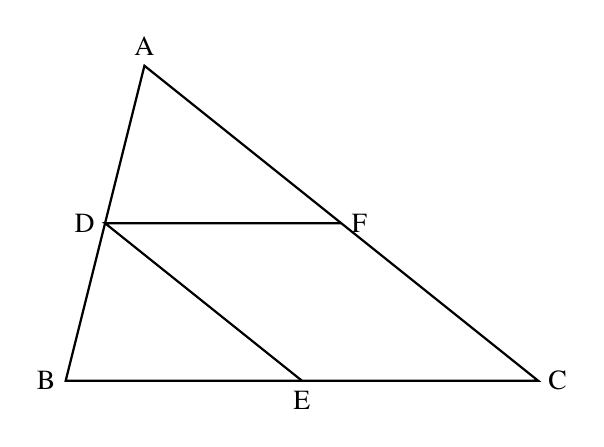
\begin{tikzpicture}[scale=1]
				\coordinate(b) at (0, 0);
				\coordinate(a) at (1, 4);
				\coordinate(c) at (6, 0);
				
				\coordinate(d) at ($(a)!0.5!(b)$);
				\coordinate(e) at ($(c)!0.5!(b)$);
				\coordinate(f) at ($(a)!0.5!(c)$);

				\draw[thick] (a)node[above]{A}--(b)node[left]{B}--(c)node[right]{C}--cycle;
				\draw[thick] (f)node[right]{F}--(d)node[left]{D}--(e)node[below]{E};

			\end{tikzpicture}
			\caption{:$\mathrm{AD}=\mathrm{DB}, \mathrm{DF}//\mathrm{BC}, \mathrm{DF}=\mathrm{BE}$}
			\label{tizk_01_ex1}
		\end{figure}

		\qpart 図\ref{tizk_01_ex2}で $\mathrm{DF}//\mathrm{BC}, \mathrm{DE}//\mathrm{AC}$である.
		このときに次の問に答えよ.

		\begin{qlist}
			\qitem $\triangle\mathrm{FEC}\equiv\triangle\mathrm{EFD}$を示せ.
			\qitem $\triangle\mathrm{DEF}$の面積が1であるとき,
			$\triangle\mathrm{ABC}$の面積がどうなるのか答えよ.
		\end{qlist}

		\begin{figure}[htbp]
			\centering
			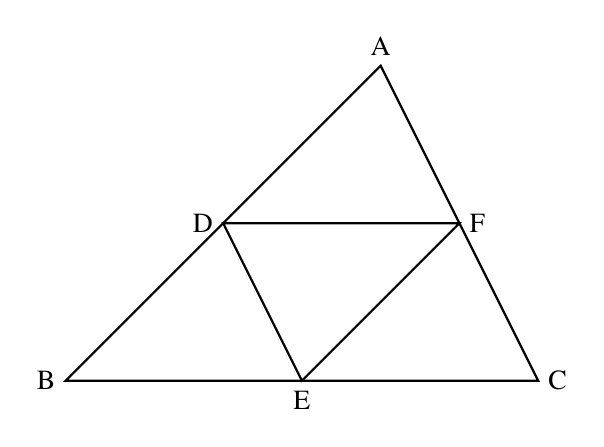
\begin{tikzpicture}[scale=1]
				\coordinate(b) at (0, 0);
				\coordinate(a) at (4, 4);
				\coordinate(c) at (6, 0);
				
				\coordinate(d) at ($(a)!0.5!(b)$);
				\coordinate(e) at ($(c)!0.5!(b)$);
				\coordinate(f) at ($(a)!0.5!(c)$);

				\draw[thick] (a)node[above]{A}--(b)node[left]{B}--(c)node[right]{C}--cycle;
				\draw[thick] (f)node[right]{F}--(d)node[left]{D}--(e)node[below]{E}--(f)--cycle;

			\end{tikzpicture}
			\caption{:$\mathrm{DF}//\mathrm{BC}, \mathrm{DE}//\mathrm{AC}$}
			\label{tizk_01_ex2}
		\end{figure}

	\end{qparts}

\end{document}




\end{document}
